%\documentclass[german,10pt]{book}      
\usepackage{makeidx}
\usepackage{babel}            % Sprachunterstuetzung
\usepackage{amsmath}          % AMS "Grundpaket"
\usepackage{amssymb,amsfonts,amsthm,amscd} 
\usepackage{mathrsfs}
\usepackage{rotating}
\usepackage{sidecap}
\usepackage{graphicx}
\usepackage{color}
\usepackage{fancybox}
\usepackage{tikz}
\usetikzlibrary{arrows,snakes,backgrounds}
\usepackage{hyperref}
\hypersetup{colorlinks=true,
                    linkcolor=blue,
                    filecolor=magenta,
                    urlcolor=cyan,
                    pdftitle={Overleaf Example},
                    pdfpagemode=FullScreen,}
%\newcommand{\hyperref}[1]{\ref{#1}}
%
\definecolor{Gray}{gray}{0.80}
\DeclareMathSymbol{,}{\mathord}{letters}{"3B}
%
\newcounter{num}
\renewcommand{\thenum}{\arabic{num}}
\newenvironment{anmerkungen}
   {\begin{list}{(\thenum)}{%
   \usecounter{num}%
   \leftmargin0pt
   \itemindent5pt
   \topsep0pt
   \labelwidth0pt}%
   }{\end{list}}
%
\renewcommand{\arraystretch}{1.15}                % in Formeln und Tabellen   
\renewcommand{\baselinestretch}{1.15}                 % 1.15 facher
                                                      % Zeilenabst.
\newcommand{\Anmerkung}[1]{{\begin{footnotesize}#1 \end{footnotesize}}\\[0.2cm]}
\newcommand{\comment}[1]{}
\setlength{\parindent}{0em}           % Nicht einruecken am Anfang der Zeile 

\setlength{\textwidth}{15.4cm}
\setlength{\textheight}{23.0cm}
\setlength{\oddsidemargin}{1.0mm} 
\setlength{\evensidemargin}{-6.5mm}
\setlength{\topmargin}{-10mm} 
\setlength{\headheight}{0mm}
\newcommand{\identity}{{\bf 1}}
%
\newcommand{\vs}{\vspace{0.3cm}}
\newcommand{\noi}{\noindent}
\newcommand{\leer}{}

\newcommand{\engl}[1]{[\textit{#1}]}
\parindent 1.2cm
\sloppy

    \begin{document}  \setcounter{chapter}{6}

\chapter{Gezeiten und Tagesl\"ange}
\index{Gezeiten}% Kap 7
\label{chap_Gezeiten2}
 
 \info{Thomas Filk}{28.03.2024}%
In diesem Kapitel wird das Ph\"anomen der Gezeiten (typischerweise zwei Flutberge
und zwei Ebbesenken am Tag, vornehmlich in Richtung des Mondes) und ihre
Entstehung vorausgesetzt (siehe hierzu den Kurztext \glqq\hyperref[chap_Gezeiten1]{Die Gezeiten -- Ebbe und Flut}\grqq). 
Es wird gezeigt, wie dieses Ph\"anomen zu einer Verlangsamung
der Erddrehung und damit zu einer Verl\"angerung der Tage f\"uhrt, und dass dies
zur Folge hat, dass sich der Mond langsam von der Erde entfernt. 

Die folgende Tabelle gibt einige Parameter an, die in diesem Kurztext ben\"otigt werden: 
\begin{table}[htb]
\begin{tabular}{r|l}
Gravitationskonstante & $G= 6,67 \cdot 10^{-11}\,{\rm \frac{m^3}{kg\cdot s^2}}$  \\  
Masse der Erde & $M_{\rm Erde} = 5,97\cdot 10^{24}$\,kg  \\ 
Masse des Monds &  $ M_{\rm Mond} =7,35 \cdot 10^{22}$\,kg  \\
Abstand Erde-Mond &  $R_{EM} = 380\,000$\,km  \\[-0.2cm] 
 & (zwischen $363\,000$ und $405\,500$\,km) \\
Erdradius &   $R_{\rm Erde} =  6\,375$\, km \\
\end{tabular}
\caption{\label{tab_Tide2}%
Einige wichtige physikalische Gr\"o\ss en im Zusammenhang mit den Gezeiten.
Da in diesem Abschnitt nur grobe Absch\"atzungen vorgenommen werden, sind die 
Werte gerundet bzw.\ gemittelt.}
\end{table}
\index{Erdmasse}\index{Mondmasse}\index{Abstand!Erde-Mond}\index{Erdradius}%
\index{Neigung der Erdachse}\index{Gravitationskonstante}

\section{Die Tage werden l\"anger}
\label{sec_EMWW}

Die Erde dreht sich einmal t\"aglich um ihre Achse. Das ist im Vergleich zu einem
Erde-Mond-Umlauf sehr schnell. Da es sich um eine Drehung um eine Achse durch
das Zentrum der Erde handelt, hat diese keinen Einfluss auf die Entstehung der Gezeiten. 
Allerdings wirken sich die Gezeiten auf diese Drehung aus: Der unebene Meeresgrund
sowie die kontinentalen K\"usten bewirken, dass es eine Reibung zwischen Erde und
Wassermassen gibt, die sogenannte Gezeitenreibung. 
Anders ausgedr\"uckt, die Wassermassen der Gezeiten treffen
auf die Ostk\"usten der Kontinente mit einer etwas gr\"o\ss eren Wucht als auf die
Westk\"usten. Dadurch wird die Erde in ihrer relativen Drehung zu den Wasserbergen
der Gezeiten abgebremst. 

Ein \"ahnlicher Effekt hat vermutlich auch dazu gef\"uhrt, dass der Mond, der urspr\"unglich
sicherlich eine Eigendrehung relativ zur Erde hatte, abgebremst wurde und mittlerweile
der Erde immer dieselbe Seite zuwendet. Hier waren es zwar keine Wassermassen, doch
durch den Gezeiteneffekt von der Erde auf den Mond wurden dort die Landmassen
leicht angehoben. Einen \"ahnlichen Effekt gibt es auch bei den Landmassen der Erde, er
macht aber nur rund 30 Zentimeter H\"ohenunterschied aus. Der Mond hat dadurch im
Verlauf der Zeit an Rotationsenergie verloren und dreht sich heute nur noch einmal im
Monat um seine Achse, wobei er der Erde immer dieselbe Seite zeigt.

\begin{figure}[htb]
\begin{tikzpicture}
\draw[thick] (3,3) circle (2.5);
\draw[->] (3,3.7) arc (90:320:0.7);
\draw[->] (11.7,3.15) -- (6.3,3.8);
\filldraw[fill=black!100] (3,3) circle (0.04);
\filldraw[fill=gray!30] (0.7,4) .. controls (0.4,3) and (0.4,2) .. (1.5,1) -- (1.5,1) .. controls (-0.2,1.7) and (-0.2,2.7) .. (0.7,4) ; \filldraw[fill=gray!30] (5.3,2) .. controls (5.6,3) and (5.6,4) .. (4.5,5) -- (4.5,5) .. controls (6.2,4.3) and (6.2,3.3) .. (5.3,2) ; 
\filldraw[fill=black!100] (5.6,3.8) circle (0.04);
\filldraw[fill=black!100] (13,3) circle (0.04);
\draw[thick] (13,3) circle (1.0);
\end{tikzpicture}
%
\caption{\label{fig_Bremsen}%
Durch die Eigendrehung der Erde relativ zu den Flutbergen kommt es zu einer
\glqq Reibung\grqq, bei der die Erde abgebremst wird, wodurch die Tage 
l\"anger werden. Andererseits haben die voreilenden Flutberge eine beschleunigende
Wirkung auf den Mond, der
dadurch an Energie gewinnt und sich von der Erde entfernt. Der Drehimpuls -- vorher
in der Eigenrotation der Erde, nachher in der Bewegung des Monds -- bleibt erhalten.}
\end{figure}

Durch die raschere Drehung der Erde werden die Wasserberge der Flut etwas
vorangetrieben, sodass diese nicht mehr auf der Verbindungslinie zwischen Erde und
Mond liegen, sondern etwas davor (siehe Abb.\ \ref{fig_Bremsen}). Auf der einen Seite
bewirkt nun die Anziehungskraft des Monds auf diese Wasserberge das Abbremsen
der Erdumdrehung, auf der anderen Seite -- im Gegenzug -- wird der Mond durch die
Anziehungskraft der Wasserberge etwas beschleunigt. Das hat einerseits den Effekt, dass
die Tage auf der Erde l\"anger werden (die Erde dreht sich langsamer -- das macht in hundert
Jahren rund 2 Millisekunden pro Tag aus, d.h.\ die Dauer eines Tages hat in den letzten 150-200
Millionen Jahren um rund eine Stunde zugenommen), andererseits\index{Tagesl\"ange, Zunahme}
nimmt der Abstand des Monds von der Erde zu. Im Jahr sind das derzeit rund 3,8 Zentimeter. 

Der Dreh\-impuls
der Erde nimmt zwar durch die Bremswirkung der Gezeiten langsam ab, aber dadurch
nimmt der Bahndrehimpuls des Monds (bzw.\ genauer des Erde-Mond-Systems) langsam
zu. Insgesamt bleibt der Gesamtdrehimpuls des Erde-Mond-Systems erhalten. 

\section{Ein paar \glqq $\pmb{\pi} \times$Daumen\grqq-Rechnungen}

\subsection{Die Zunahme der Tagesl\"ange}

Der Drehimpuls des Erde-Mond-Systems steckt in erster Linie in der
Mondbahn (Drehung des Monds um den gemeinsamen Schwerpunkt) und
in zweiter Linie in der Eigendrehung der Erde. Der Bahndrehimpuls der Erde und die
Eigendrehung des Monds k\"onnen vernachl\"assigt werden. Tabelle \ref{tab_Drehimpuls} gibt
einige Gr\"o\ss enordnungen an. Die Bahndrehimpulse von Erde und Mond berechnen
sich nach\index{Drehimpuls}
\begin{equation}
\label{eq_Bahndrehimpuls}
             L_{\rm Bahn} = m r v = m r^2 \omega = m r^2 \frac{2\pi}{T} \, ,
\end{equation}
($m$ die Masse des Objekts, $r$ der Abstand Schwerpunkt-Mittelpunkt des Objekts, $v$ die 
Geschwindigkeit des Objekts, $\omega$ die zugeh\"orige Winkelgeschwindigkeit).\footnote{
Das Verh\"altnis der Drehimpulse von Erd- zu Mondbahn l\"asst sich einfacher absch\"atzen:
F\"ur den Schwerpunkt des Erde-Mond-Systems gilt 
$m_{\rm Erde} R_{\rm Erde-D}=m_{\rm Mond} R_{\rm Mond-D}$,
wobei $R_{\rm X-D}$ der Abstand des Mittelpunkts des K\"orpers $X$ zum gemeinsamen Schwerpunkt
$D$ ist. Die Winkelgeschwindigkeit ist f\"ur die beiden K\"orper im Erde-Mond-System dieselbe, also
erhalten wir die Gleichung\index{Drehimpuls!Erde-Mond-System}
\[   m_{\rm Erde} R_{\rm Erde} \omega = m_{\rm Mond} R_{\rm Mond}  \omega \, .\]
Diese ist gleichbedeutend zu
\[   R_{\rm Erde} L_{\rm Erde/Bahn} =  R_{\rm Mond} L_{\rm Mond/Bahn} \]
oder auch
\[   m_{\rm Mond} L_{\rm Erde/Bahn} =  m_{\rm Erde} L_{\rm Mond/Bahn}  \, .\]
Das Verh\"altnis der Bahndrehimpulse ist also gleich dem umgekehrten Verh\"altnis der Massen.
Dieses ist immer gleich (es betr\"agt ungef\"ahr $1:81,2$), daher ist auch das Verh\"altnis der Bahndrehimpulse 
unabh\"angig vom Abstand zwischen Erde und Mond. } 
Die Umlaufperiode $T$ ist die siderische Periode der Mondbahn, das sind ungef\"ahr 27,3 Tage.
Die Eigendrehimpulse wurden nach\index{Drehimpuls!Vollkugel}
\begin{equation}
\label{eq_Eigendrehimpuls}
             L_{\rm Eigen} = \frac{2}{5}  m R^2 \omega \, ,
\end{equation}
berechnet ($m$ Masse, $R$ Radius des Objekts, $\omega$ bzw.\ $T$ die Eigenfrequenz
bzw.\ Periode der Drehung; f\"ur den Mond ist $T=27,3$\,Tage, f\"ur die Erde ist $T=1$\,Tag oder
86\,400\,Sekunden). Hier wird die Annahme gemacht, dass die Masse der Objekte konstant 
verteilt ist, es sich also um eine starre Vollkugel handelt. Dies ist insbesondere f\"ur die Erde
mit ihrem fl\"ussigen Erdinneren nicht wirklich gegeben, stellt aber eine gute N\"aherung dar. 

\begin{table}[htb]
\begin{tabular}{r|l|l}
System & Drehimpuls & prozentualer Anteil \\ \hline
Mondbahn um Schwerpunkt & $ 2,83 \cdot 10^{34}\, {\rm kg\cdot m^2/s}$ & $79$\% \\  
Erdbahn um Schwerpunkt & $  3,4 \cdot 10^{32}\, {\rm kg\cdot m^2/s} $ & $1$\%\\ 
Eigendrehung Erde &  $ 7,06 \cdot 10^{33}\, {\rm kg\cdot m^2/s} $ & $19,9$\% \\
Eigendrehung Mond &  $ 2,4 \cdot 10^{29} \, {\rm kg\cdot m^2/s}  $ & $<0,001$\% \\
\end{tabular}
\index{Mondbahn!Drehimpuls}\index{Drehimpuls!Mondbahn}\index{Erdbahn!Drehimpuls}\index{Drehimpuls!Erdbahn}%
\index{Erde!Drehimpuls}\index{Mond!Drehimpuls}%
\caption{\label{tab_Drehimpuls}%
Gr\"o\ss enordnung der Drehimpulse im Erde-Mond-System. Die Zahlen sind wiederum nur
ungef\"ahre Angaben und wurden aus den Parametern in Tab.\ \ref{tab_Tide2} berechnet. 
Unsicherheiten liegen in der Annahme einer Kreisbahn f\"ur den
Mond sowie in der Formel f\"ur die Eigendrehimpulse, die eine konstante Masseverteilung
voraussetzt. Insbesondere ist der Eigendrehimpuls der Erde etwas kleiner (ungef\"ahr 
$5,85\cdot 10^{33}\, {\rm kg\cdot m^2/s}$). Damit erh\"oht sich der Anteil des Bahndrehimpulses des
Monds im Vergleich zum Gesamtdrehimpuls auf rund 82\%, entsprechend verringert
sich der Anteil des Eigendrehimpulses der Erde auf rund 17\%. 
}
\end{table}

Wenn nun die Eigendrehung der Erde aufgrund der Gezeitenreibung abnimmt, flie\ss t
dieser Drehimpuls praktisch ausnahmslos in den Bahndrehimpuls des Monds. Die Summe
der \"Anderungen verschwindet und wir k\"onnen
annehmen, dass
\begin{equation}
          \frac{\Delta L_{\rm Erde/Eigen}}{\Delta t} = -  \frac{\Delta L_{\rm Mond/Bahn}}{\Delta t}  \, .
\end{equation}
Im Grenzfall $\Delta t \rightarrow 0$ wird dieser Quotient zum Drehmoment. 

Wir kennen das Drehmoment der Gezeitenreibung nicht. Aber wir kennen ziemlich genau
den Abstand Erde-Mond und wissen, dass der Abstand des Monds im Laufe eines Jahres
um rund 3,8\,cm zunimmt. Bevor wir diesen Wert in Gl.\ \ref{eq_Bahndrehimpuls} einsetzen
m\"ussen wir ber\"ucksichtigen, dass eine \"Anderung des Abstands (bzw.\ des Bahnradius)
auch eine \"Anderung der Umlaufzeit zur Folge hat. Aus der Bedingung \glqq Gravitationskraft = Fliehkraft\grqq\
(korrekterweise sollte man nat\"urlich sagen \glqq Gravitationskraft = Impuls\"anderung bei einer
Kreisbewegung \grqq) folgt:
\begin{equation}
         G \frac{m_{\rm Erde} m_{\rm Mond}}{R_{EM}^2} = m_{\rm Mond} R_{\rm EM} \left( \frac{2\pi}{T} \right)^2  
          \hspace{0.8cm} \Longrightarrow \hspace{0.8cm}
          T =2 \pi  \left(  \frac{R_{\rm EM}^3}{G m_{\rm Erde}}   \right)^{1/2} \, .
\end{equation}
Dies ist das ber\"uhmte dritte Kepler'sche Gesetz: Die Quadrate der Umlaufzeiten verhalten sich wie
die Kuben der Halbachsen. Setzen wir diese Beziehung\index{Kepler'sche Gesetze!drittes} 
in Gl.\ \ref{eq_Bahndrehimpuls} ein, erhalten wir den Drehimpuls der Mondumlaufbahn
als Funktion des Abstands (sowie weiterer Konstanten):
\begin{equation}
\label{eq_BahnMond}
        L_{\rm Mond/Bahn} = m_{\rm Mond} \sqrt{G m_{\rm Erde} R_{\rm EM}} \, .
\end{equation}
Die \"Anderung des Drehimpulses als Funktion des Abstands ist somit:\hyperref[secB]{(Herleitung)}
\begin{equation}
        \Delta L_{\rm Mond/Bahn} = \frac{m_{\rm Mond}}{2} \sqrt{ \frac{G m_{\rm Erde}}{R_{\rm EM}}} \Delta R \, .
\end{equation}
F\"ur $\Delta R = 3,8$\,cm ist dies die Drehimpuls\"anderung in der Mondbahn in einem Jahr. 
Um denselben Wert \"andert sich der Eigendrehimpuls der Erde in einem Jahr. Da sich in Gl.\ \ref{eq_Eigendrehimpuls}
nur $\omega$ \"andern kann, folgt:
\begin{equation}
        \Delta L_{\rm Erde/Eigen} = \frac{2}{5} m_{\rm Erde} R_{\rm Erde}^2 \Delta \omega =
            - \frac{2}{5} m_{\rm Erde} R_{\rm Erde}^2 \frac{2 \pi }{T^2} \Delta T \, .
\end{equation}
(Hier wurde $\Delta \omega = \frac{{\rm d}\omega}{{\rm d}T} \Delta T$ ausgenutzt.) Das Minuszeichen deutet
an, dass der Drehimpuls kleiner wird (also $\Delta L$ negativ ist) wenn die Periode l\"anger wird (also $\Delta T$
positiv ist).  Insgesamt erhalten wir somit:
\begin{equation}
       \Delta T = \frac{5}{8 \pi} T^2  
                \frac{m_{\rm Mond}}{m_{\rm Erde}R_{\rm Erde}^2} \sqrt{ \frac{G m_{\rm Erde}}{R_{\rm EM}}} \Delta R \, .
\end{equation}
Mit den Gleichungen f\"ur den Bahndrehimpuls des Monds (Gl.\ \ref{eq_BahnMond}) und dem Eigendrehimpuls
der Erde (Gl.\ \ref{eq_Eigendrehimpuls}) k\"onnen wir diese Beziehung auch umschreiben:
\begin{equation}
\label{eq_DeltaDelta}
      \frac{ \Delta T}{T}  = \frac{1}{2}  
                \frac{L_{\rm Mond/Bahn}}{L_{\rm Erde/Eigen}} \frac{\Delta R}{R_{\rm EM}} \, .
\end{equation}
Diese Beziehung besitzt eine \glqq rasche\grqq\ Herleitung: Wir wissen, dass
\begin{equation}
\label{eq_SumDeltaL}
                \Delta L_{\rm Erde/Eigen} + \Delta L_{\rm Mond/Bahn} = 0  \, .
\end{equation}
Die beiden Relationen
\begin{equation}
       L_{\rm Erde/Eigen} \propto \frac{1}{T}  \hspace{1cm} {\rm und} \hspace{1cm}  
       L_{\rm Mond/Bahn} \propto  \sqrt{R_{\rm EM}}  
\end{equation}
f\"uhren auf (man bilde jeweils die logarithmischen Ableitungen, sodass die Proportionalit\"atsfaktoren wegfallen)
\begin{equation}
       \Delta L_{\rm Erde/Eigen} = - \frac{L_{\rm Erde/Eigen}}{T} \Delta T   \hspace{1cm} {\rm und} \hspace{1cm}  
       \Delta L_{\rm Mond/Bahn} =  \frac{1}{2} \frac{L_{\rm Mond/Bahn}}{R_{\rm EM}} \Delta R_{\rm EM} 
\end{equation}
Eingesetzt in Gl.\ \ref{eq_SumDeltaL} erhalten wir Gl.\ \ref{eq_DeltaDelta}. Nach Tabelle \ref{tab_Drehimpuls}
ist $\frac{L_{\rm Mond/Bahn}}{L_{\rm Erde/Eigen}} \approx 4$, au\ss erdem ist $\frac{\Delta R_{\rm EM}}{R_{\rm EM}}
\approx 10^{-10}$ und $T=86\,400$\,s. Damit folgt
\begin{equation}
             \Delta T =  2 \cdot 10^{-10} \cdot 0,864 \cdot 10^5\,{\rm s} \approx 1,7 \cdot 10^{-5} \,{\rm s} \, .  
\end{equation}
Dies ist die \"Anderung in der Tagesl\"ange in einem Jahr. In 100 Jahren sind das etwas weniger als
$0,002$\,s. 

\subsection{Wie alt ist der Mond?}

Die Frage nach dem Alter des Monds ist f\"ur viele Bereiche von Bedeutung.\index{Mondalter} 
Die Vermutung
ist, dass der Mond vor rund 4,5 Milliarden Jahren, also kurz nach der Entstehung der Erde, durch
einen Zusammensto\ss\ mit einem kleineren Planeten entstanden ist. 
Wenn wir ganz naiv die 3,8\,cm 
pro Jahr, um die die Entfernung des Monds von der Erde zunimmt, extrapolieren, kommen wir
bei 4 Milliarden Jahren auf eine Entfernung von rund $1,52 \cdot 10^8$\,m oder $152\,000$\,km. 
Diese Entfernung ist deutlich zu gro\ss. Vermutlich hatte der Mond kurz nach seiner Entstehung
eine Entfernung von der Erde, die knapp \"uber der Grenze lag, bei welcher der Mond aufgrund
der Gezeitenkr\"afte auseinandergerissen worden w\"are (diese Grenze bezeichnet man auch als
Roche-Grenze), das sind rund 15\,000-20\,000\,km.\index{Roche-Grenze} 

Es ist offensichtlich, weshalb die naive Extrapolation der 3,8\,cm pro Jahr f\"ur die Zunahme
der Erde-Mond-Entfernung nicht korrekt ist. Mehrere Gr\"unde spielen hier eine wichtige Rolle.
Insbesondere muss ber\"ucksichtigt werden, dass der Abstand zwischen Erde und Mond
fr\"uher kleiner war. 
\begin{enumerate}
\item
Damit folgt, dass die Gezeitenkr\"afte, die sich wie $1/R_{\rm EM}^3$ verhalten, wesentlich
gr\"o\ss er waren. Bei einem gro\ss z\"ugig angenommenen Faktor 10 zwischen dem urspr\"unglichen
Abstand und dem heutigen Abstand macht dies f\"ur die Gezeitenkr\"afte einen Faktor 1000 aus. 
Dieser Einfluss auf Ebbe und Flut l\"asst sich kaum absch\"atzen.
\item
Ein kleinerer Abstand zwischen Erde und Mond bedeutet auch, dass sich der Mond wesentlich
schneller um die Erde gedreht hat. Nimmt man auch hier einen Faktor 10 an, folgt aus dem dritten
Kepler'schen Gesetz, dass die Mondzyklen um mehr als einen Faktor 30 k\"urzer waren als heute,
der Mond sich also in weniger als einem (heutigen) Tag um die Erde gedreht hat. Damit war
auch die Zeitdauer zwischen Ebbe und Flut deutlich k\"urzer.
\item
Schlie\ss lich hat sich die Erde fr\"uher wesentlich schneller gedreht als heute und damit
folgten Ebbe und Flut rascher aufeinander. Der Reibungseffekt pro Jahr war wegen der
h\"aufigeren Fluten (unabh\"angig von ihrer St\"arke) h\"oher.
\end{enumerate} 
Ber\"ucksichtigt man all diese Effekte, so hat sich der Mond insbesondere zu Beginn deutlich
schneller von der Erde entfernt, als es unsere naive Extrapolation angibt. Eine Rechnung, die
all diese Effekte ber\"ucksichtigt, kommt auf ein Alter des Monds von rund 1,37 Milliarden 
Jahren (siehe \cite{DeYoung}).

Dies wiederum ist eine zu kurze Zeitdauer. Dieses Ergebnis wird gelegentlich von Creationisten
(Anh\"angern einer auf der Darstellung der Bibel basierenden Sch\"opfungsgeschichte, nach der
Gott die Welt von etwas \"uber 6000 Jahren erschaffen hat) angef\"uhrt um zu argumentieren, dass
die sogenannten wissenschaftlichen Berechnungen f\"ur das Alter der Erde (und des Monds), die 
auf etwas \"uber 4,5 Milliarden Jahre deuten, falsch sein m\"ussen. 
Sie sehen hierin einen Widerspruch zu den beobachteten Tatsachen.

W\"are das Ergebnis von 1,37 Milliarden Jahren f\"ur das Alter des Monds korrekt, w\"are das
tats\"achlich ein Problem f\"ur die \"ubliche wissenschaftliche Theorie \"uber das Alter der Erde.
Der wesentliche Unsicherheitsfaktor f\"ur die obige Berechnung ist jedoch der Einfluss der um einen
Faktor 10--1000 (als Gr\"o\ss enordnung) st\"arkeren Gezeitenkr\"afte auf Ebbe und Flut und die 
damit verbundene Gezeitenreibung. Insbesondere wird vermutet, dass die Gezeitenreibung in
fr\"uheren Jahrmillionen einen deutlich geringeren Einfluss hatte, als eine einfache Extrapolation
von heutigen Verh\"altnissen vermuten lie\ss e: Es gab vor rund 200 Millionen Jahren nur einen gro\ss en
Kontinent (Pangaea), und vermutlich gab es in der Geschichte der Erde vor ein bzw.\ zwei Milliarden
Jahren mehrere Phasen, in denen es nur einen Kontinent gab. Dadurch war die Gezeitenreibung
deutlich geringer (es gab weniger K\"usten) und der Effekt des Dreh\-impulsaustauschs zwischen Erde
und Mond war wesentlich kleiner. Hier gibt es noch viele Unsicherheiten, das Argument der
Creationisten ist jedoch sicherlich zu einfach und nicht haltbar.

\subsection{Wie geht es weiter?}

Die Erde wird sich in Zukunft immer langsamer drehen und der Mond dabei immer mehr
entfernen. Die Monate werden dadurch ebenfalls l\"anger. Ist der derzeitige Eigendrehimpuls
(siehe Tab.\ \ref{tab_Drehimpuls}) der Erde \glqq aufgebraucht\grqq\ und ganz auf den Mond \"ubergegangen,
wird der Mond einen Bahndrehimpuls von rund $3,54\cdot 10^{34}$\,km$\cdot$m/s${}^2$ haben.
Nach Gl.\ \ref{eq_BahnMond} bedeutet dies einen Abstand Erde-Mond von etwas \"uber 
$R_{\rm EM}=425\,000\,{\rm km}$ und der Monat wird rund 33 (heutige) Sonnentage dauern.   
Die Rotation der Erde ist dann an den Mond gebunden, so wie jetzt schon die Rotation des
Monds gebunden ist, d.h.\ der Mond zeigt der Erde immer dieselbe Seite. Daher dauert ein Monat
dann nur einen Sonnentag. 

\begin{thebibliography}{9}
\bibitem{DeYoung} DeYoung, D.B.; \textit{The Earth-Moon System}, in The Proceedings of the
          International Conference on Creationism; Vol.\ 2:II; p. 79--84.  
\end{thebibliography}

\section{Herleitung einiger Gleichungen}

\subsection{Differenzieller Drehimpuls}
\label{secB}

Der direkte Weg, aus 
\begin{equation}
        L_{\rm Mond/Bahn}(R_{\rm EM}) = m_{\rm Mond} \sqrt{G m_{\rm Erde} R_{\rm EM}} 
\end{equation}
das Differenzial zu $L$ abzuleiten, ist die Taylor-Entwicklung bzw.\ die erste Ableitung:
\begin{equation}
       \frac{{\rm d} L_{\rm Mond/Bahn}(R_{\rm EM})}{{\rm d}R_{\rm EM}} = 
          \frac{1}{2} m_{\rm Mond} \sqrt{\frac{G m_{\rm Erde}}{R_{\rm EM}}} 
\end{equation}
und somit folgt:
\begin{equation}
       \Delta  L_{\rm Mond/Bahn}(R_{\rm EM}) = 
          \frac{1}{2} m_{\rm Mond} \sqrt{\frac{G m_{\rm Erde}}{R_{\rm EM}}} \Delta R \, .
\end{equation}

Man kann die Ableitung auch umgehen:
\begin{eqnarray}
        \Delta L_{\rm Mond/Bahn} & \equiv &   L_{\rm Mond/Bahn}(R_{\rm EM}+\Delta R) -  L_{\rm Mond/Bahn}(R_{\rm EM}) \\
        &=& m_{\rm Mond} \sqrt{G m_{\rm Erde} ( R_{\rm EM} + \Delta R)} - m_{\rm Mond} \sqrt{G m_{\rm Erde} R_{\rm EM}}
          \, .
\end{eqnarray}
Wir klammern $R_{\rm EM}$ aus:
\begin{eqnarray}
        \Delta L_{\rm Mond/Bahn}
        &=&  m_{\rm Mond} \sqrt{G m_{\rm Erde} R_{\rm EM} \left( 1 + \frac{\Delta R}{R_{\rm EM}}\right) }  
                   - m_{\rm Mond} \sqrt{G m_{\rm Erde} R_{\rm EM}}  \\
      &=& m_{\rm Mond} \sqrt{G m_{\rm Erde} R_{\rm EM}} \left( \sqrt{1 + \frac{\Delta R}{R_{\rm EM}} } - 1 \right)               
\end{eqnarray}
Wir nutzen nun die Entwicklung der Wurzelfunktion:
\begin{equation}
        \sqrt{1+ x} \approx 1 + \frac{1}{2} x + O(x^2)  
\end{equation}
und erhalten:
\begin{equation}
        \Delta L_{\rm Mond/Bahn}
        =\frac{1}{2} m_{\rm Mond} \sqrt{G m_{\rm Erde} R_{\rm EM}} ~   \frac{\Delta R}{R_{\rm EM}} 
        =\frac{1}{2} m_{\rm Mond} \sqrt{\frac{G m_{\rm Erde}}{R_{\rm EM}}} ~   \Delta R \, .
\end{equation}

%\end{document}
